\documentclass[a4paper,fleqn]{cas-sc}

% Elsevier CAS template; target journal: Simulation Modelling Practice and Theory.
\usepackage[T1]{fontenc}
\usepackage[utf8]{inputenc}
\usepackage[english]{babel}
\usepackage[authoryear]{natbib}
\usepackage{amsmath,amssymb}
\usepackage{graphicx}
\usepackage{tikz}
\usetikzlibrary{positioning,fit,arrows.meta}
\usepackage{booktabs}
\usepackage{array}
\usepackage{float}
\usepackage{xcolor}
\usepackage{microtype}
\microtypesetup{expansion=false}
\IfFileExists{xurl.sty}{\usepackage{xurl}}{\usepackage{url}}
\setlength{\emergencystretch}{3em}
\hyphenation{inter-community intra-community Gillespie}

\floatstyle{ruled}
\newfloat{algorithm}{tbp}{loa}
\floatname{algorithm}{Algorithm}
\floatstyle{plain}
\restylefloat{figure}
\restylefloat{table}

\newtheorem{proposition}{Proposition}
\newtheorem{corollary}{Corollary}
\newdefinition{remark}{Remark}
\newproof{proof}{Proof}

\newcommand{\ibar}{\bar{y}}
\newcommand{\sbar}{\bar{s}}
\newcommand{\Exp}{\mathrm{Exp}}
\newcommand{\Full}{\textup{\textsc{Full}}}
\newcommand{\TS}{\textup{\textsc{TwoScale}}}
\newcommand{\ind}{\mathbf{1}}
\newcommand{\eW}{e_{W}}

% Suppress the CAS abstract heading in this sections-only document.
\RenewDocumentEnvironment{Abstract}{o}{}{}
% Later-section reference numbers are preserved for this partial manuscript.
\AtBeginDocument{\input{final_en_sections_1_3_20261009/later_sections_labels.tex}}
\begin{document}
\let\WriteBookmarks\relax
\def\floatpagepagefraction{1}
\def\textpagefraction{.001}

\shorttitle{Two-scale stochastic simulation with aggregate inter-community coupling}
\shortauthors{Y. Kuryliak and M.T.M. Emmerich}

\title[mode=title]{Two-scale stochastic simulation of epidemics on community networks with aggregate inter-community coupling}

\author[1]{Yulian Kuryliak}[orcid=0000-0002-6600-2637]
\cormark[1]
\ead{yulian.a.kuryliak@lpnu.ua}
\affiliation[1]{organization={Institute of Computer Science and Information Technologies, Lviv Polytechnic National University},
            addressline={12 Stepan Bandera Street},
            city={Lviv},
            postcode={79000},
            country={Ukraine}}

\author[2]{Michael T. M. Emmerich}[orcid=0000-0002-7342-2090]
\ead{michael.t.m.emmerich@jyu.fi}
\affiliation[2]{organization={Faculty of Information Technology, University of Jyv\"askyl\"a},
            addressline={P.O. Box 35 (Agora)},
            city={Jyv\"askyl\"a},
            postcode={FI-40014},
            country={Finland}}

\cortext[1]{Corresponding author}

\maketitle

% English translation of the user's saved Ukrainian Sections 1--3.
% Original baseline: claude-version_merged_parallel_EN.tex.
\begingroup\color{black}
\hypersetup{citecolor=black,linkcolor=black}

%======================================================================
\section{Introduction}
\label{sec:introduction}

Epidemics spread at more than one scale. Inside a community, infection may pass through a detailed network of contacts between people \citep{keeling2005,pastorsatorras2015,kiss2017}. Between communities, the available data are often much less detailed. For example, they may give only passenger numbers, commuting flows, or a weighted link between two places \citep{balcan2009,barbosa2018human}. We therefore need a model that can use a detailed network inside each community and simpler data between communities.

This situation is common in practice. A local contact network may be observed, reconstructed, or generated to match known properties such as clustering and mean shortest-path length \citep{eubank2004,danon2011}. In contrast, links between communities may be known only through transport, migration, commuting, or mobile-phone data \citep{barbosa2018human,chang2021}. Such data can tell us the total strength of connection between two communities, but not which people form the connection. We may therefore know the total coupling without knowing the bridge nodes or their infection states.

If every contact is known, a continuous-time Markov chain (CTMC) can describe the epidemic, and a Gillespie-type method can simulate it exactly \citep{gillespie1977exact,gibson2000}. Efficient methods are also available for temporal, large, and sparse networks \citep{vestergaard2015,kuryliak2025simulating}. However, these methods still need the individual contacts that may transmit infection. Metapopulation models use aggregate flows between communities, but usually also replace the detailed local network by population counts \citep{colizza2007reaction,colizza2008,balcan2010modeling,ajelli2010}. Our problem lies between these two cases: we want to keep node-level stochastic spread inside every community while using only aggregate information between communities.

The idea of a two-scale simulator was presented in an earlier conference paper \citep{kuryliak2025towards}. It runs a separate local simulator for each community. The macro layer uses the current community states and connection weights to generate infections arriving from another community. In this article, we describe the method in detail and study its approximation error. In particular, we examine what is lost when real cross-community edges and their endpoints are replaced by the total connection weight, and an imported infection is placed on a randomly selected susceptible node.

Our main question is: when is this aggregate connection sufficient to reproduce the quantity of interest in the full-network CTMC? We study infection arrival times, their distributions, and whether transmission is possible through the real contacts. Similar arrival times do not guarantee a possible transmission route: the two-scale model can infect another community while all real bridge nodes in the source community are still susceptible. To test this, we use synthetic networks in which every contact is known. Full-network Gillespie simulation receives the whole network, whereas the two-scale method receives only the local networks and the total weights of the cross-community connections.

This article makes four contributions.
\begin{enumerate}
\item We describe how the simulator works: each community is simulated separately, and a shared scheduler determines infections between them. We explain how it coordinates the local simulators on time intervals of fixed length (Section~\ref{sec:method}, Algorithm~\ref{alg:scheduler}).
\item We show which network the method simulates exactly. It is exact for a \emph{surrogate network}: the real cross-community edges are replaced by weak connections between all node pairs, preserving the total weight (Proposition~\ref*{prop:surrogate}). We then identify the sources of error and analyse a single export of infection (Proposition~\ref*{prop:ordering}).
\item We compare the two-scale method with full-network Gillespie simulation for transmission to one neighbouring community and for spread along chains of communities. We measure differences using the relative shift in the median time of first infection and the Wasserstein distance between the distributions of these times (Sections~\ref*{sec:design} and~\ref*{sec:results}).
\item We propose an empirical indicator of accuracy for our benchmarks. It compares the spread of infection times inside a community with the typical transmission time through one cross-community edge (Section~\ref*{sec:res_descriptor}).
\end{enumerate}

We consider susceptible--infected (SI) dynamics on static synthetic networks and use one fixed synchronisation step. Section~\ref{sec:related} explains the relation to earlier methods. Section~\ref{sec:method} describes the simulator. Section~\ref*{sec:analysis} explains what the aggregate interface preserves and loses. Sections~\ref*{sec:design} and~\ref*{sec:results} present the experiments and results. Section~\ref*{sec:discussion} discusses use, cost, and limitations.

\clearpage

%======================================================================
\section{Related work}
\label{sec:related}

\paragraph{Simulation of stochastic events.}
Gillespie's direct method draws the next event and its time from the current event rates \citep{gillespie1977exact}. The next reaction method keeps a separate clock for each possible event \citep{gibson2000}. Both methods are exact for the CTMC they simulate. When an event rate changes with time, its rate can be accumulated until it reaches a random threshold \citep{ethier1986}. \citet{anderson2007} used this idea for systems with time-dependent rates and delays. Our macro clock uses the same idea, but its rate changes because the local epidemic states change. Network simulators can save work by updating only the rates affected by the latest event \citep{vestergaard2015,kuryliak2025simulating}. Our local simulators use the implementation of \citet{kuryliak2025simulating}.

Some multiscale methods speed up chemical-reaction models by approximating reactions that occur much faster than others \citep{haseltine2002,cao2005slow}. Our method removes a different kind of detail. It keeps the local infection events, but does not know which individual cross-community edges are currently able to transmit. Even so, the relative speeds of local spread and cross-community transmission help explain its error.

\paragraph{Models with several communities.}
Metapopulation models represent each subpopulation by counts and connect the subpopulations by mobility flows. They have been used to study global spread and the conditions for invasion \citep{colizza2007reaction,colizza2008,balcan2009,balcan2010modeling}. Detailed mobility data can also be combined with local transmission models \citep{chang2021}. Agent-based models instead represent individuals throughout the model \citep{eubank2004,kerr2021}. \citet{ajelli2010} compared these two broad approaches. The method studied here keeps individual nodes and contacts inside each community, but replaces the unknown individual contacts between communities by one aggregate stochastic interface.

\paragraph{Two levels of mixing and co-simulation.}
Some epidemic models combine contacts in small local groups with uniform mixing at a wider level \citep{ball1997}. Our surrogate network is related to this idea, but uniform mixing is used only between connected pairs of communities, and its strength is set by their aggregate weight.

The implementation also has features of co-simulation. In co-simulation, separate subsystem solvers move forward on a shared time grid and exchange a limited amount of information \citep{gomes2018cosim}. Here, the local community simulators are those subsystems. They send their infected and susceptible counts to the macro layer. In this implementation, those exchanged counts are used to draw a cross-community infection time and then to choose its receiving community and target node. The scheduler can therefore treat the local simulators as black boxes.

\clearpage

%======================================================================
\section{The two-scale simulation method}
\label{sec:method}

The experiments use one implementation of the two-scale simulator, in which the local simulators exchange information with the macro scheduler at fixed time intervals. To understand its error, we also consider a process with the same rates but exact timing of every event. We call this theoretical description the \emph{ideal process}. It separates the error caused by changing the network from the additional error caused by the time grid. The ideal process is exact for the surrogate network defined later; this does not make it exact for the original physical network. Below, we explain the reference model, the available data, and the steps of the implemented simulator.

\subsection{Full-network reference model}
\label{sec:reference}

Let $G=(V,E)$ be the contact network. Its nodes are divided into $M$ non-overlapping communities:
\begin{equation}
\label{eq:partition}
V=V_1\cup V_2\cup\cdots\cup V_M,
\qquad N_i=|V_i|.
\end{equation}
Here, $V_i$ is the node set of community $i$, and $N_i$ is its size. We write $E_{ii}$ for contacts inside community $i$ and $E_{ij}$ for contacts from nodes in community $i$ to nodes in community $j$. We treat each contact as an oriented transmission channel. An undirected contact therefore gives two channels, one in each direction.

Every node is susceptible ($S$), infected ($I$), or removed ($R$). The full network state at time $t$ is $X(t)$, and the state of community $i$ is $X_i(t)$. Let $S_i(t)$ and $I_i(t)$ be the sets of susceptible and infected nodes in that community. Their sizes are $s_i(t)$ and $y_i(t)$, and their fractions are $\sbar_i(t)=s_i(t)/N_i$ and $\ibar_i(t)=y_i(t)/N_i$. Below, $x$ denotes a particular network state; $x^{v:I}$ is the same state after node $v$ becomes infected, and $x^{u:R}$ is the state after node $u$ is removed.

The full model follows two simple rules. A susceptible node $v$ receives infection from each infected neighbour $u$ at rate $\beta_{uv}$. An infected node is removed at rate $\gamma$. We can write both rules as
\begin{equation}
\label{eq:full_generator}
q_v(x)=\sum_{\substack{u:(u,v)\in E\\x_u=I}}\beta_{uv}
\quad (x_v=S),
\qquad r_u(x)=\gamma\quad (x_u=I).
\end{equation}
Here, $q_v$ is the total infection rate of node $v$, and $r_u$ is the removal rate of node $u$. For a non-susceptible node, $q_v=0$; for a non-infected node, $r_u=0$. A rate describes how often an event occurs: for a constant rate $q$, the mean waiting time is $1/q$. For a cross-community channel, we write $\beta_{uv}=\beta_{\mathrm{out}}w_{uv}$, where $w_{uv}$ is its contact weight. We call exact simulation of these full-network rates \Full{}. All experiments in this article use SI dynamics, so $\gamma=0$.

The waiting time between state transitions is exponential and is determined by the total rate of all events in the current state $x$, which is
\[
a(x)=\sum_v q_v(x)+\sum_u r_u(x).
\]
If $a(x)>0$, the waiting time to the next event is exponentially distributed with rate $a(x)$ and mean $1/a(x)$. Infection of node $v$ is selected with probability $q_v(x)/a(x)$, and removal of node $u$ with probability $r_u(x)/a(x)$. After the event, the rates are updated. If $a(x)=0$, no further event can occur.

\subsection{Aggregate interface}
\label{sec:interface}

The two-scale simulator, denoted \TS{}, knows every local graph $G_i=(V_i,E_{ii})$ and its rates. It does not know the individual cross-community channels in $E_{ij}$. For each ordered pair of communities, it knows only the total weight
\begin{equation}
\label{eq:weight}
W_{ij}=\sum_{(u,v)\in E_{ij}}w_{uv},
\qquad i\neq j.
\end{equation}
If all weights equal one, $W_{ij}$ is the number of directed channels from $V_i$ to $V_j$. In an application, this total may instead come from transport, migration, mobility, or contact data. The macro layer also receives the current susceptible and infected counts from each local simulator. It does not know which nodes are endpoints of real cross-community edges. Table~\ref{tab:information} gives the main difference, and Figure~\ref{fig:schematic} shows it visually.

\begin{table}[tbp]
\color{black}
\centering
\caption{\textcolor{black}{Information used by the two models. The ``target rule'' in \TS{} is uniform among susceptible nodes in all experiments in this article.}}
\label{tab:information}
\small
\begin{tabular}{>{\raggedright\arraybackslash}p{0.42\linewidth}>{\raggedright\arraybackslash}p{0.23\linewidth}>{\raggedright\arraybackslash}p{0.25\linewidth}}
\toprule
Information or action & \Full{} & \TS{}\\
\midrule
Local contacts, rates, and node states & known & known by local simulators\\
Individual cross-community edges and bridge nodes & known & unknown\\
Total cross-community weight $W_{ij}$ & obtained from the edges & given directly\\
Cross-community event rate & uses states of real edge endpoints & uses $\ibar_i$, $\sbar_j$, and $W_{ij}$\\
Target of a cross-community infection & endpoint of the active edge & a susceptible node drawn by the target rule\\
Number of possible SI infections through one bundle & at most the number of its channels & at most $s_j$ target infections\\
\bottomrule
\end{tabular}
\end{table}

\begin{figure}[tbp]
\color{black}
\centering
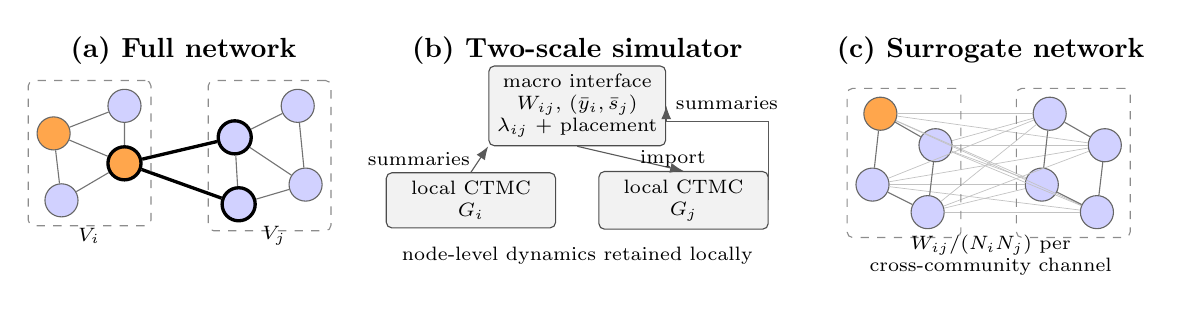
\begin{tikzpicture}[
  x=1cm,y=1cm,
  font=\scriptsize,
  >=Latex,
  person/.style={circle,draw=black!60,fill=blue!18,minimum size=4.2mm,inner sep=0pt},
  infected/.style={person,fill=orange!70},
  bridge/.style={person,very thick,draw=black},
  bridgeinf/.style={infected,very thick,draw=black},
  commbox/.style={draw=black!45,dashed,rounded corners=2pt,inner sep=3pt},
  macrobox/.style={draw=black!70,rounded corners=2pt,fill=black!5,align=center,inner sep=3pt},
  link/.style={draw=black!55},
  weak/.style={draw=black!24,line width=.25pt},
  flow/.style={-{Latex[length=1.7mm]},draw=black!65}
]
% (a) Full microscopic interface
\node[font=\bfseries] at (0,2.25) {(a) Full network};
\node[infected] (a1) at (-1.65,1.20) {};
\node[person]   (a2) at (-1.55,0.35) {};
\node[bridgeinf](a3) at (-0.75,0.82) {};
\node[person]   (a4) at (-0.75,1.55) {};
\node[bridge]   (b1) at (0.65,1.15) {};
\node[person]   (b2) at (1.45,1.55) {};
\node[person]   (b3) at (1.55,0.55) {};
\node[bridge]   (b4) at (0.70,0.30) {};
\draw[link] (a1)--(a2)--(a3)--(a1) (a1)--(a4)--(a3);
\draw[link] (b1)--(b2)--(b3)--(b4)--(b1) (b1)--(b3);
\draw[very thick] (a3)--(b1);
\draw[very thick] (a3)--(b4);
\node[commbox,fit=(a1)(a2)(a3)(a4)] {};
\node[commbox,fit=(b1)(b2)(b3)(b4)] {};
\node at (-1.2,-0.10) {$V_i$};
\node at (1.15,-0.10) {$V_j$};

% (b) Two-scale representation
\node[font=\bfseries] at (5.0,2.25) {(b) Two-scale simulator};
\node[macrobox] (macro) at (5.0,1.55) {macro interface\\$W_{ij}$, $(\ibar_i,\sbar_j)$\\$\lambda_{ij}$ + placement};
\node[macrobox,minimum width=2.15cm,minimum height=.70cm] (li) at (3.65,0.35) {local CTMC\\$G_i$};
\node[macrobox,minimum width=2.15cm,minimum height=.70cm] (lj) at (6.35,0.35) {local CTMC\\$G_j$};
\draw[flow] (li.north) -- node[left] {summaries} (macro.south west);
\draw[flow] (macro.south) -- node[right] {import} (lj.north);
\draw[flow] (lj.east) -- ++(0,1.0) -| node[pos=1.08,right] {summaries} (macro.east);
\node at (5.0,-0.35) {node-level dynamics retained locally};

% (c) Surrogate interface
\node[font=\bfseries] at (10.25,2.25) {(c) Surrogate network};
\node[infected] (c1) at (8.85,1.45) {};
\node[person]   (c2) at (8.75,0.55) {};
\node[person]   (c3) at (9.55,1.05) {};
\node[person]   (c4) at (9.45,0.20) {};
\node[person]   (d1) at (11.00,1.45) {};
\node[person]   (d2) at (10.90,0.55) {};
\node[person]   (d3) at (11.70,1.05) {};
\node[person]   (d4) at (11.60,0.20) {};
\foreach \u in {c1,c2,c3,c4}{\foreach \v in {d1,d2,d3,d4}{\draw[weak] (\u)--(\v);}}
\draw[link] (c1)--(c2)--(c4)--(c3)--(c1);
\draw[link] (d1)--(d2)--(d4)--(d3)--(d1);
\node[commbox,fit=(c1)(c2)(c3)(c4)] {};
\node[commbox,fit=(d1)(d2)(d3)(d4)] {};
\node[align=center] at (10.25,-0.35) {$W_{ij}/(N_iN_j)$ per\\cross-community channel};
\end{tikzpicture}
\caption{\textcolor{black}{Three views of the interface. (a) In the full network, infection can cross only through the shown physical edges and their bridge nodes. (b) The two-scale simulator keeps a separate local simulator for each community. The macro layer receives community counts, uses $W_{ij}$ to generate a cross-community infection, and places it on a uniformly selected susceptible node. (c) The ideal two-scale process is equivalent to a surrogate network in which every ordered node pair across the two communities has a weak connection. The connections together have total weight $W_{ij}$. Orange nodes are infected and blue nodes are susceptible.}}
\label{fig:schematic}
\end{figure}

\subsection{Local simulators}
\label{sec:local}

Each community has a separate Gillespie simulator for its local graph $G_i$. It applies the infection and removal rates in~\eqref{eq:full_generator} using only the local edges $E_{ii}$. The implementation updates only rates affected by the latest event, following \citet{kuryliak2025simulating}. Each local simulator is independent and has its own random-number stream.

The macro layer can advance a local simulator to a specified time. The simulator applies the local events up to that time. The macro layer can then import an infection by changing one selected susceptible node to $I$. This changes the local rates. The implementation keeps the unused part of the random threshold for the next local event and recalculates its waiting time using the new total rate.

To recalculate the time of the next local event after an import, the simulator retains the remaining random threshold. Let $E_{\mathrm{loc}}\sim\mathrm{Exp}(1)$ be the threshold drawn after the previous local event, and let $A_{\mathrm{loc}}$ be the integral of the total local rate from that event to the import time. After the import, the total local rate is $a_{\mathrm{new}}$. If $a_{\mathrm{new}}>0$, the remaining waiting time is
\[
\Delta t=
\frac{E_{\mathrm{loc}}-A_{\mathrm{loc}}}{a_{\mathrm{new}}}.
\]
Thus, an import changes the waiting time, but not the random threshold itself. If another import occurs first, the accumulated rate is updated and the waiting time is recalculated again. If $a_{\mathrm{new}}=0$, no local event can occur until the rate becomes positive.

The event type and its node are selected using the updated rates. A new local threshold is drawn only if there is no existing one. Each local clock has its own threshold, separate from the macro threshold described in Section~\ref{sec:timing}. For prescribed import times and target nodes, the local simulator follows the CTMC rules of its own network. The approximation comes from the way imports are generated and their target nodes are selected.

\subsection{Macro layer}
\label{sec:macro}

The macro layer represents each community by its current fractions and represents each directed connection by $W_{ij}$. Its rate for an infection from community $i$ to community $j$ is
\begin{equation}
\label{eq:macro_rate}
\lambda_{ij}(t)=\beta_{\mathrm{out}}W_{ij}\ibar_i(t)\sbar_j(t),
\qquad
\Theta(t)=\sum_{i\neq j}\lambda_{ij}(t).
\end{equation}
The factors have a direct meaning: $\beta_{\mathrm{out}}W_{ij}$ gives the total connection strength, $\ibar_i$ is the infected fraction in the source, and $\sbar_j$ is the susceptible fraction in the receiving community. The sum $\Theta$ is the rate of any cross-community infection. Calculating the waiting time to the next event when $\Theta$ varies with time requires special treatment (Section~\ref{sec:timing}).

When such an event occurs, first select the source and receiving communities $(i,j)$ with probability $\lambda_{ij}/\Theta$. Then choose one susceptible node uniformly in the receiving community $j$ and infect it. If there are 20 susceptible nodes, each has probability $1/20$. This selection does not use real bridge nodes, because the aggregate interface does not know them. In later formulas, we write this target probability as $\Pi_{ij}(v\mid x)=1/s_j$ for $v\in S_j$, where $x$ is the current network state. Thus, $\Pi$ simply denotes the probability of choosing a particular susceptible node. Other target rules can be used if bridge-node information is available.

This aggregate rate is generally an approximation to transmission through the real physical edges. For fixed community counts, it is the expected rate under uniformly random selection of the edge endpoints, before their particular identities, states, and epidemic history are taken into account. This does not guarantee the correct rate for an epidemic already realised on specific edges. For uniform all-to-all coupling, it is the actual rate, as explained in Section~\ref*{sec:analysis}.

\subsection{Timing and synchronisation}
\label{sec:timing}

After a macro event at time $t_0$, draw a random threshold $E\sim\Exp(1)$: an exponential random number with mean one. Starting from zero, accumulate the total macro rate $\Theta$:
\begin{equation}
\label{eq:hazard_integral}
A(t)=\int_{t_0}^{t}\Theta(s)\,ds,
\qquad A(t_0)=0.
\end{equation}
The next macro event occurs at the first time $t^\ast$ when $A(t^\ast)=E$.

In words, the area under the rate curve grows until it first reaches the random threshold. If it never reaches the threshold, no further macro event occurs. This is the standard cumulative-rate construction \citep{ethier1986,anderson2007}. If $\Theta$ is constant, the waiting time is $E/\Theta$. Drawing $E=-\ln U$, with $U$ uniform on $(0,1)$, gives the familiar Gillespie waiting time. When $\Theta$ changes after a local event, we keep the same threshold and continue accumulating with the new rate. We draw a new macro threshold only after a macro event. Exact calculation of its first crossing defines the ideal process; the time-grid calculation below approximates that crossing. Section~\ref*{sec:surrogate} shows that the ideal process is exact for the surrogate network.

The scheduler divides time into intervals of length $\tau$. On each interval, it approximates the varying macro rate by its value at the midpoint. Let $A$ be the amount already accumulated since the previous macro event. For the current interval $[t,t_g)$, copy every local simulator, including its random-number state, and advance each copy to the midpoint. The copies give an estimate $\Theta_{\mathrm{mid}}$ of the total macro rate. The estimated increase over the remaining interval is $\Theta_{\mathrm{mid}}(t_g-t)$. If $A$ plus this increase is below $E$ (the random macro threshold), the real simulators move to $t_g$. Otherwise, estimate the event time by
\begin{equation}
\label{eq:interpolation}
t^\ast=t+\frac{E-A}{\Theta_{\mathrm{mid}}}.
\end{equation}
Here, $E$ is the random macro threshold and $A$ is the amount already accumulated toward it. The numerator $E-A$ is what remains; dividing by the estimated rate gives the remaining waiting time. For example, if $E=1$, $A=0.4$, and $\Theta_{\mathrm{mid}}=0.2$, the estimated wait is three time units. The scheduler advances the real simulators to $t^\ast$, selects the source and receiving communities using their states at that time, chooses the susceptible target, and imports the infection. Algorithm~\ref{alg:scheduler} gives the full sequence.

\begin{algorithm}[H]
\color{black}
\caption{\textcolor{black}{Grid-synchronised two-scale simulation of one realisation.}}
\label{alg:scheduler}
\small
\fbox{\begin{minipage}{0.94\linewidth}
\textbf{Input:} local graphs $G_i$, weights $W_{ij}$, rates, step $\tau$, horizon $T_{\mathrm{end}}$, and initial state.
\begin{enumerate}
\item Set $t=0$ and accumulated rate $A=0$; draw $E\sim\Exp(1)$.
\item While $t<T_{\mathrm{end}}$ and infection can still spread, set $t_g=\min(t+\tau,T_{\mathrm{end}})$ and process the interval up to $t_g$.
\item Copy every local simulator, including its random-number state. Advance the copies to the midpoint of the remaining interval and calculate $\Theta_{\mathrm{mid}}$ from~\eqref{eq:macro_rate}.
\item If $A+\Theta_{\mathrm{mid}}(t_g-t)<E$, advance the real simulators to $t_g$, add this amount to $A$, set $t=t_g$, and return to step 2.
\item Otherwise, calculate $t^\ast$ from~\eqref{eq:interpolation} and advance the real simulators to $t^\ast$.
\item Select $(i,j)$ with probability $\lambda_{ij}(t^\ast)/\Theta(t^\ast)$. Select $v$ uniformly from $S_j(t^\ast)$ and import infection at $v$. Update the receiving local simulator, keeping its unused exponential threshold and selecting the local event from the new rates.
\item Set $t=t^\ast$ and $A=0$, draw a new $E\sim\Exp(1)$, and process the rest of the current interval in the same way.
\end{enumerate}
\end{minipage}}
\end{algorithm}

The copied random-number states are important. Unless an import occurs first, a copied simulator follows the same path that the real simulator will follow to the midpoint. The midpoint estimate is exact on an interval with no local event. Its timing error and its look-ahead of at most $\tau/2$ decrease to zero as $\tau$ decreases.

The time grid is needed because the scheduler treats local simulators as black boxes. If they also report their next local-event times, the scheduler can merge those times and accumulate the piecewise-constant value of $\Theta$ exactly. That event-driven version removes the numerical synchronisation approximation. The experiments in this article use the implemented grid version with $\tau=1$.

\subsection{Computational structure and intended use}
\label{sec:cost}

\Full{} stores all local and cross-community channels, and its work per event grows with node degree \citep{kuryliak2025simulating}. \TS{} stores the local graphs and an $M\times M$ matrix of aggregate weights. The conference paper discusses this reduction in the information stored for cross-community contacts \citep{kuryliak2025towards}. Its importance depends on the problem. Replacing many individual cross-community edges by one weight can reduce storage. If only a few such edges exist, this saving may be small, and the local graphs still have to be stored.

The separate local simulators also provide an opportunity for parallel execution. Once the scheduler has chosen the next target time ($t_g$ or $t^\ast$), the local simulators can advance independently to that same time. The midpoint copies can also be processed in parallel. The macro layer must then collect the counts and apply any scheduled import before continuing. The implementation studied here advances the local simulators sequentially; parallel execution within one run is a possible extension, not a measured speedup. Local simulators can also use different community-specific settings.

The grid scheduler adds work by copying local states and coordinating the communities. Therefore, neither lower memory use nor faster execution is guaranteed. The method is useful when individual cross-community contacts are unavailable or too numerous to represent explicitly.

\clearpage
\endgroup

\bibliographystyle{cas-model2-names}
\bibliography{twoscale_references}
\end{document}
